%%%%%%%%%%%%%%%%%%%%%%%%%%%%%%%%%%%%%%%%%
% Jacobs Landscape Poster
% LaTeX Template
% Version 1.0 (29/03/13)
%
% Created by:
% Computational Physics and Biophysics Group, Jacobs University
% https://teamwork.jacobs-university.de:8443/confluence/display/CoPandBiG/LaTeX+Poster
% 
% Further modified by:
% Nathaniel Johnston (nathaniel@njohnston.ca)
%
% This template has been downloaded from:
% http://www.LaTeXTemplates.com
%
% 
% Masaryk University presentation themes were downloaded from:
% https://www.overleaf.com/gallery/tagged/muni
%
% and ported into Jacobs Landscape Poster by:
% Jumaidil Awal (ideal1st.here@googlemail.com)
% 
% Jacobs Landscape Poster License:
% CC BY-NC-SA 3.0 (http://creativecommons.org/licenses/by-nc-sa/3.0/)
%
% Masaryk University's fibeamer theme license:
% Copyright 2015  Vít Novotný <witiko@mail.muni.cz>
% Faculty of Informatics, Masaryk University (Brno, Czech Republic)
% under Latex Project Public License
%
%%%%%%%%%%%%%%%%%%%%%%%%%%%%%%%%%%%%%%%%%

%----------------------------------------------------------------------------------------
%	PACKAGES AND OTHER DOCUMENT CONFIGURATIONS
%----------------------------------------------------------------------------------------

\documentclass[final]{beamer}

\usepackage[scale=1.24]{beamerposter} % Use the beamerposter package for laying out the poster

%\usetheme{confposter} % Use the confposter theme supplied with this template
\usetheme[faculty=chemo]{fibeamer} % Uncomment to use Masaryk University's fibeamer theme instead.

%\setbeamercolor{block title}{fg=ngreen,bg=white} % Colors of the block titles
%\setbeamercolor{block body}{fg=black,bg=white} % Colors of the body of blocks
%\setbeamercolor{block alerted title}{fg=white,bg=dblue!70} % Colors of the highlighted block titles
%\setbeamercolor{block alerted body}{fg=black,bg=dblue!10} % Colors of the body of highlighted blocks
% Many more colors are available for use in beamerthemeconfposter.sty

%-----------------------------------------------------------
% Define the column widths and overall poster size
% To set effective sepwid, onecolwid and twocolwid values, first choose how many columns you want and how much separation you want between columns
% In this template, the separation width chosen is 0.024 of the paper width and a 4-column layout
% onecolwid should therefore be (1-(# of columns+1)*sepwid)/# of columns e.g. (1-(4+1)*0.024)/4 = 0.22
% Set twocolwid to be (2*onecolwid)+sepwid = 0.464
% Set threecolwid to be (3*onecolwid)+2*sepwid = 0.708

\newlength{\sepwid}
\newlength{\onecolwid}
\newlength{\twocolwid}
\newlength{\threecolwid}
\setlength{\paperwidth}{46.8in} % A0 width: 46.8in
\setlength{\paperheight}{33.1in} % A0 height: 33.1in
\setlength{\sepwid}{0.024\paperwidth} % Separation width (white space) between columns
\setlength{\onecolwid}{0.21\paperwidth} % Width of one column
\setlength{\twocolwid}{0.451\paperwidth} % Width of two columns
\setlength{\threecolwid}{0.678\paperwidth} % Width of three columns
%\setlength{\topmargin}{-0.5in} % Reduce the top margin size
%-----------------------------------------------------------

\usepackage{graphicx}  % Required for including images

\usepackage{booktabs} % Top and bottom rules for tables

%----------------------------------------------------------------------------------------
%	TITLE SECTION 
%----------------------------------------------------------------------------------------

\title{F10 : Standard Deviation Function} % Poster title

\author{Nayana Raj Cheluvaraju (40071318, Team-B)} % Author(s)

\institute{Concordia University, Montreal} % Institution(s)

%----------------------------------------------------------------------------------------

\begin{document}
\addtobeamertemplate{block end}{}{\vspace*{2ex}} % White space under blocks
\addtobeamertemplate{block example end}{}{\vspace*{2ex}} % White space under example blocks
\addtobeamertemplate{block alerted end}{}{\vspace*{2ex}} % White space under highlighted (alert) blocks

\setlength{\belowcaptionskip}{2ex} % White space under figures
\setlength\belowdisplayshortskip{2ex} % White space under equations
%\begin{darkframes} % Uncomment for dark theme, don't forget to \end{darkframes}
\begin{frame} % The whole poster is enclosed in one beamer frame

%==========================Begin Head===============================

  \begin{columns}
   \begin{column}{\linewidth}
    \vskip1cm
    \centering
    \usebeamercolor{title in headline}{\color{fg}\Huge{\textbf{\inserttitle}}\\[0.5ex]}
    \usebeamercolor{author in headline}{\color{fg}\Large{\insertauthor}\\[1ex]}
    \usebeamercolor{institute in headline}{\color{fg}\large{\insertinstitute}\\[1ex]}
    \vskip1cm
   \end{column}
   \vspace{1cm}
  \end{columns}
 \vspace{1cm}

%==========================End Head===============================

\begin{columns}[t] % The whole poster consists of three major columns, the second of which is split into two columns twice - the [t] option aligns each column's content to the top

\begin{column}{\sepwid}\end{column} % Empty spacer column

\begin{column}{\onecolwid} % The first column

%----------------------------------------------------------------------------------------
%	OBJECTIVES
%----------------------------------------------------------------------------------------

\begin{exampleblock}{Iterations overview}

\begin{itemize}
\item All tasks were completed on time.
\item Calculator was developed exclusive for Standard deviation function.
\item The calculator has graphical user interface(GUI).
\end{itemize}

\end{exampleblock}

%----------------------------------------------------------------------------------------
%	INTRODUCTION
%----------------------------------------------------------------------------------------

\begin{exampleblock}{Standard Deviation (SD) Function}
Measures extent of variation or separation of data values. The symbol $\sigma$ notifies SD. The Range for standard deviation is between negative infinity to positive infinity. There are Two types:\newline
\textbf{1. Population Standard Deviation}
\newline
Used when an entire population can be measured.
\begin{center}
\begin{math}
\sigma=\sqrt{\frac{1}{N}\Sigma_{i=1}^{N}(x_{i}-\mu)^2}
\end{math}
\end{center}
\newline
\textbf{2. Sample Standard Deviation}
\newline
Measured through random samples of the population. 
\begin{center}
\begin{math}
s= \sqrt{\frac{1}{N-1}\Sigma_{i=1}^{N}(x_{i}-\bar{x})^2}
\end{math}
\end{center}
\end{exampleblock}

%----------------------------------------------------------------------------------------
%	OBJECTIVES
%----------------------------------------------------------------------------------------

\begin{exampleblock}{Process Followed}
\begin{figure}
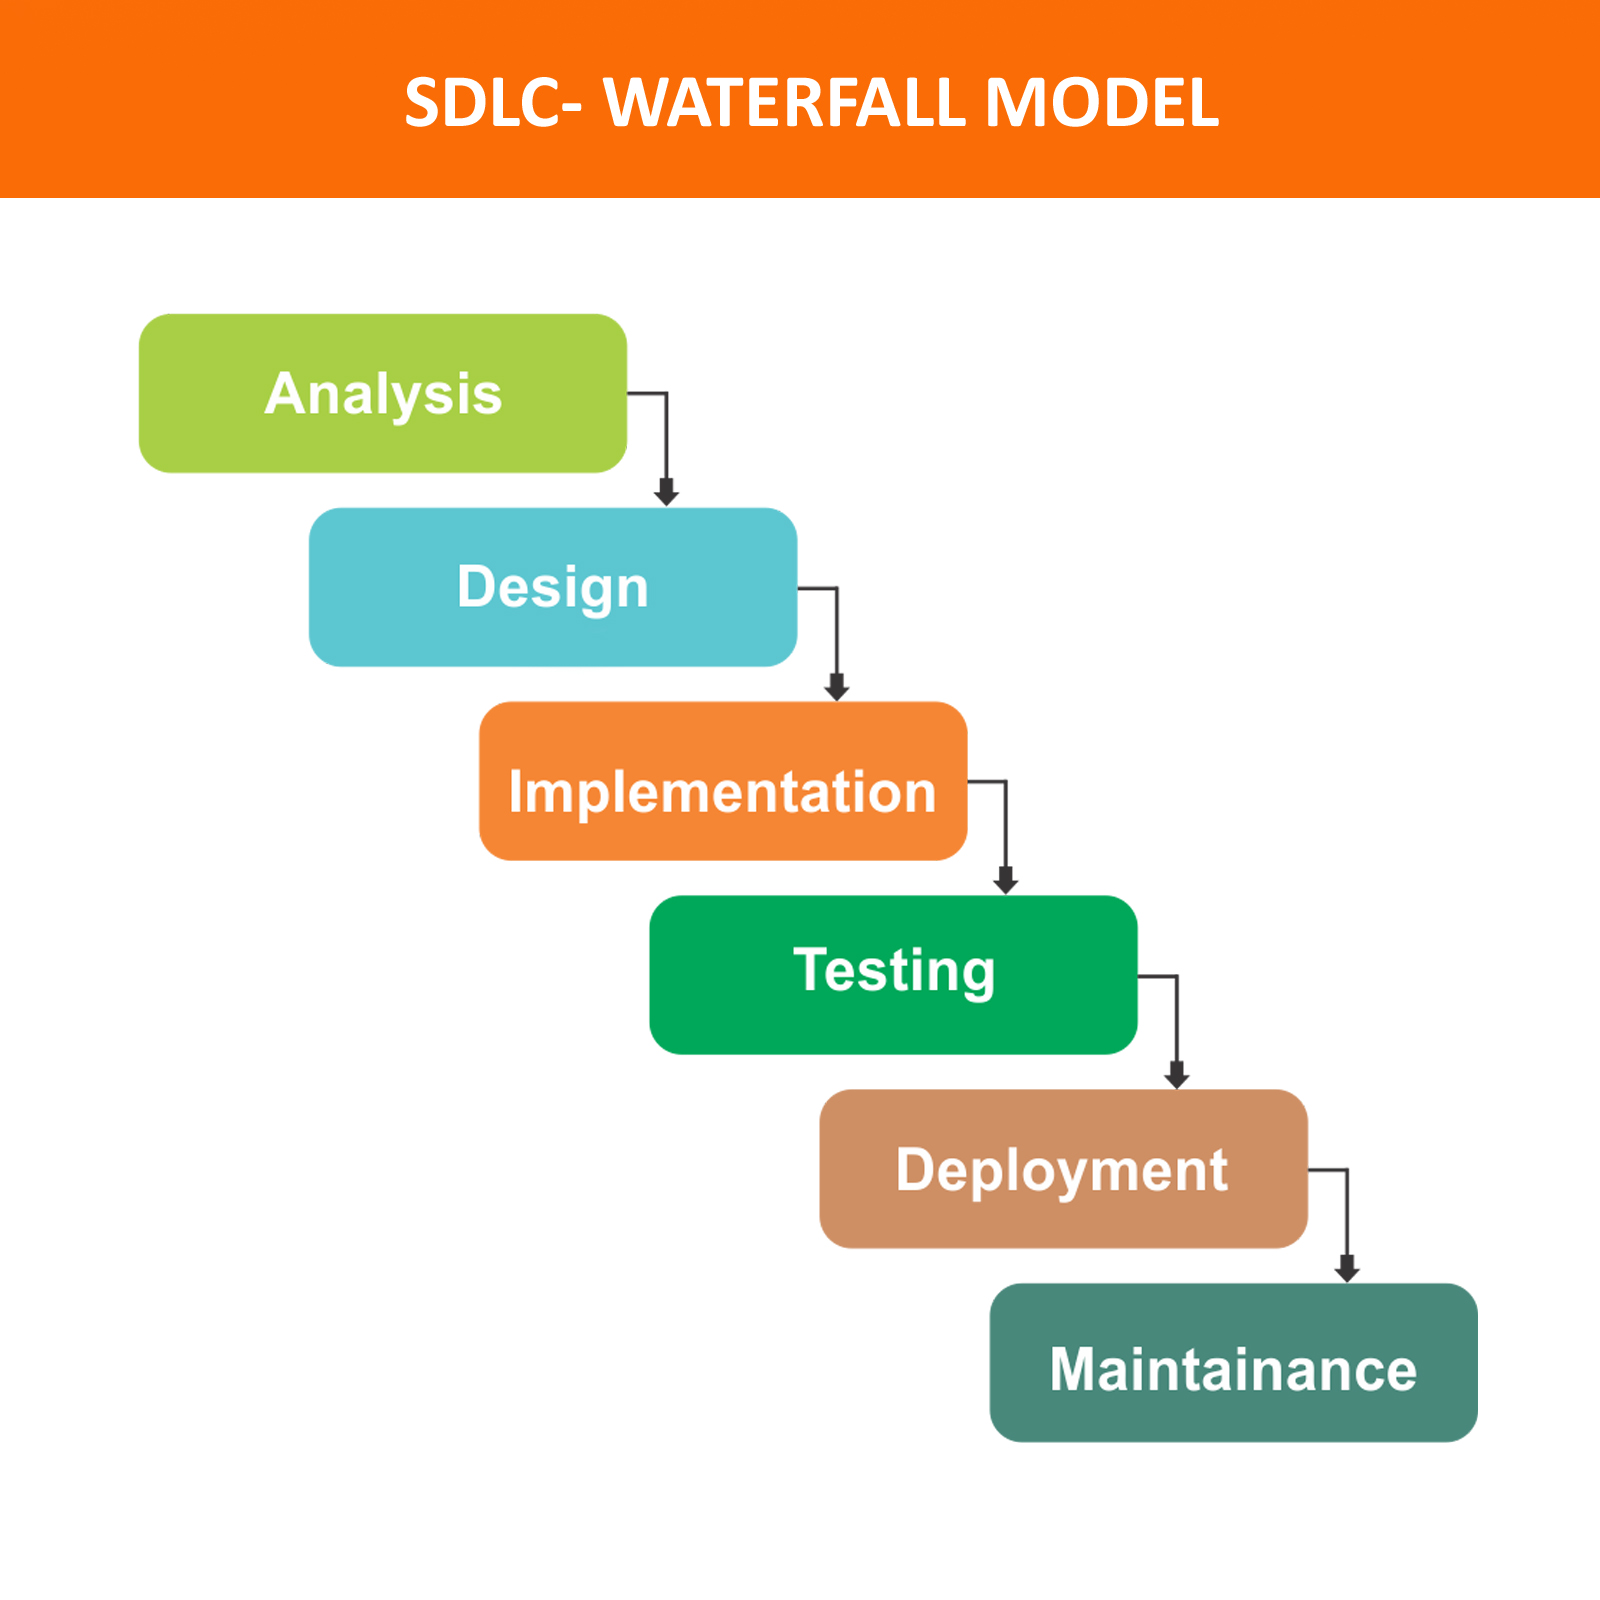
\includegraphics[width=1\linewidth]{waterfall-jpg.jpg}
\end{figure}
\end{exampleblock}

%----------------------------------------------------------------------------------------

\end{column} % End of the first column

\begin{column}{\sepwid}\end{column} % Empty spacer column

\begin{column}{\twocolwid} % Begin a column which is two columns wide (column 2)

\begin{columns}[t,totalwidth=\twocolwid] % Split up the two columns wide column

\begin{column}{\onecolwid}\vspace{-.74in} % The first column within column 2 (column 2.1)

%----------------------------------------------------------------------------------------
%	Critical Decision
%----------------------------------------------------------------------------------------

\begin{exampleblock}{Critical Decisions Made}
\begin{itemize}
\item Making the calculator exclusively for Standard deviation function.\\
\textbf{Why is this critical?}\\
The reason to have only one function was to give basic working function and user should not get confused with other functions. 

\item   There was limited time to decide between Test based or GUI.\\
\textbf{Why is this critical?}\\
As there was change in deadline for submission, had to decide whether to submit text based or implement GUI. The text-based version was not seeming to be much effective, so within overnight developed GUI.

\item Not rounding of result up to certain(2 or 3) decimal place.\\
\textbf{Why is this critical?}\\
Standard deviation function is used in stock market, measure risk, real estate etc.. If we do not consider the value till the last decimal point the actual values might vary in larger number, so no option to round off decimal point.

\end{itemize}
\end{exampleblock}
%----------------------------------------------------------------------------------------
%	CONCLUSION
%----------------------------------------------------------------------------------------

\begin{exampleblock}{Lessons Learnt}
\begin{itemize}
\item Working in \textbf{latex}.
\item Building function without using \textbf{Math libraries}.
\item Java swings for \textbf{graphical user interface}.
\item \textbf{Systematic way of programming}: Using coding standards/coding convention
\item Using \textbf{tools} : Junit, checkstyle,  PMD
\item Benefits of code review  and testing.
\end{itemize}
\end{exampleblock}

%----------------------------------------------------------------------------------------

\end{column} % End of column 2.1
\begin{column}{\sepwid}\end{column} % Empty spacer column

\begin{column}{\onecolwid}\vspace{-.74in} % The second column within column 2 (column 2.2)

%----------------------------------------------------------------------------------------
%	What did not go well and how can we improve
%----------------------------------------------------------------------------------------

\begin{exampleblock}{What did not go well and how can we improve}
\begin{itemize}
\item Users are not given change to select precision.\\
\textbf{How to improve?}\\
Giving option to select the number, to make number as last decimal point to be rounded.
\item Not giving option to save previous calculation history. \\
\textbf{How to improve?}\\
Using separate button for history and developing it to store last three calculation results.
\item One-line commented code or missed comments in the code. \\
\textbf{How to improve?}\\
By writing Javadoc in more descriptive way so that others can easily understand the code and also write comments for missed return parameter.
\item Improvising Graphical user Interface. \\
\textbf{How to improve?}\\
Find the suitable user interface design pattern and implement same.

\end{itemize}
\end{exampleblock}
%----------------------------------------------------------------------------------------
%	MATHEMATICAL SECTION
%----------------------------------------------------------------------------------------
\begin{exampleblock}{Future work}

\begin{itemize}
\item Incorporating calculator to have multiple functions.
\item User will able to choose precision level, i.e points up to  what decimal point the user want result to be. 
\item Calculator will have history button.
\item Implementing with user Interface design pattern.
\item Improvising GUI with better color and options. 
\end{itemize}

\end{exampleblock}

%----------------------------------------------------------------------------------------

\end{column} % End of column 2.2

\end{columns} % End of the split of column 2 - any content after this will now take up 2 columns width

%----------------------------------------------------------------------------------------

%----------------------------------------------------------------------------------------

\begin{columns}[t,totalwidth=\twocolwid] % Split up the two columns wide column again

\begin{column}{\onecolwid} % The first column within column 2 (column 2.1)

%----------------------------------------------------------------------------------------

%----------------------------------------------------------------------------------------

\end{column} % End of column 2.1
\begin{column}{\sepwid}\end{column} % Empty spacer column

\begin{column}{\onecolwid} % The second column within column 2 (column 2.2)

%----------------------------------------------------------------------------------------
%	RESULTS
%----------------------------------------------------------------------------------------


%----------------------------------------------------------------------------------------

\end{column} % End of column 2.2

\end{columns} % End of the split of column 2

\end{column} % End of the second column

\begin{column}{\sepwid}\end{column} % Empty spacer column

\begin{column}{\onecolwid} % The third column

%----------------------------------------------------------------------------------------
%	CONCLUSION
%----------------------------------------------------------------------------------------

\begin{exampleblock}{Graphical User Interface}
\begin{figure}
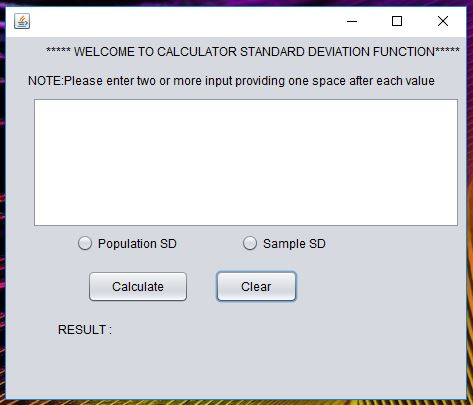
\includegraphics[width=1\linewidth]{GUI.JPG}\\
Figure: Screenshot of GUI developed \\
\end{figure}
Java swings is used to develop GUI. User has to provide input values, select radio button (for population or sample SD)and clicks on calculate. The result is displayed in result section. 
\end{exampleblock}

%----------------------------------------------------------------------------------------
%	REFERENCES
%----------------------------------------------------------------------------------------

\begin{exampleblock}{References}
\begin{itemize}
\item [1] https://www.mathsisfun.com/data/standard-deviation-formulas.html\\
\item [2] https://www.overleaf.com/ \\
\end{itemize}
\end{exampleblock}

%----------------------------------------------------------------------------------------
%	ACKNOWLEDGEMENTS
%----------------------------------------------------------------------------------------

%\setbeamercolor{block title}{fg=red,bg=white} % Change the block title color

%\begin{exampleblock}{Acknowledgements}

%\small{\rmfamily{Nam mollis tristique neque eu luctus. Suspendisse rutrum congue nisi sed convallis. Aenean id neque dolor. Pellentesque habitant morbi tristique senectus et netus et malesuada fames ac turpis egestas.}} \\

%\end{exampleblock}

%----------------------------------------------------------------------------------------
%	CONTACT INFORMATION
%----------------------------------------------------------------------------------------

%\setbeamercolor{block alerted title}{fg=black,bg=norange} % Change the alert block title colors
%\setbeamercolor{block alerted body}{fg=black,bg=white} % Change the alert block body colors

\begin{block}{GitHub Information}

$https://github.com/nayanarajc/SOEN_6011$ \newline
username: nayanarajc
\end{block}

\begin{block}{Guided By}
\textbf{ Dr. P.kamthan}
\end{block}
\begin{tabular}{rr}
\hspace{0.5\linewidth} & 
\includegraphics[width=0.4\linewidth]{Concordia-Logo1.jpg}
\end{tabular}

%----------------------------------------------------------------------------------------

\end{column} % End of the third column

\begin{column}{\sepwid}\end{column} % Empty spacer column

\end{columns} % End of all the columns in the poster

\end{frame} % End of the enclosing frame
%\end{darkframes} % Uncomment for dark theme
\end{document}
